\section{Background and Motivation}
HER MÅ JEG OGSÅ HA MED AT SOM NEVNT I ABSTRACT, MÅ VI GJENNOM FLERE STEG. NESTE STEG ER Å DESIGNE EN SENSORBÆRENDE PLATFORM SOM KAN BRUKE DETEKSJONSMETODENE. 
\\\\
A good way to work with materials, identify them or learn about their properties, is to study how light interacts with them - spectroscopy, which by definition examines how light behaves in the target and recognizes materials based on their different spectral signatures (which can be identified from the spectrum), while the spectrum describes the amount of light in different wavelengths, showing how much light is reflected, emitted and transmitted from the target. In other words, the spectrum simply shows how much of a certain color the light contains. 
Spectral signatures can be compared to fingerprints. While fingerprints often is used to identify i person, spectral signatures can be used to identify materials. One of the purposes of this study, is to identify different types of plastic using their spectral signatures. 

%Development of hyperspectral imaging as a bio-optical taxonomic tool for pigmented marine organisms - geir
Former studies on marine organisms have shown that reflectance signatures obtained from HI and UHI are inversely related to the specific absorption signature of the organism (Volent et al. 2007, 2009)

\\\\
The research questions driving this project are centered around whether micro plastics and their spectral signatures in fact can be separated from other material and microorganisms. Do different types of plastics leave different spectral signatures? Could a signature change as the sea tears the plastic pieces? Is it possible that the spectral signatures differ in different environments?

\subsection{Background Andreas}
%What is plastic - Will be related to the recognition, social context, the possibilities it has resulted in, its chemical structure, chemical properties, various types

\subsubsection{General} %Mulig dette også er hakket for kort. Kan være en ide å utfylle mer på hva plasten er. Se over om det er egenskaper ved plasten som påpekes og som burde nevnes i teorien.
The following paragraph is largely inspired by \citet{Callister2007MaterialsBy}.\\ %Referansen må spesifisere sidetall også
Plastic is a term used in a wide range of fields to describe properties and behaviour of materials, in addition to the common type of materials. The report will use the term plastic solely with the purpose of describing the types of materials.
\\
\\
Plastic are organic polymers based on carbon, hydrogen and other nonmetallic elements commonly produced from crude oil or naturally occurring. The molecular structures are large with a backbone of carbon atoms, where the chains have several thousand repeating units. The materials typically have low densities, with mechanical properties different from metallic and ceramic materials. Plastics are usually less stiff and weaker than metals and ceramics. However, on account of the strength and stiffness per mass the plastics are comparable. The combination of strength, weight and ductility has made the material extremely popular, with it being used in everything from food wrapping to prostheses. The properties of plastic highly vary depending on the type and the side chains of the basic polymer structure and the additives blended into most plastics. The latter could potentially be highly toxic and the source of the toxicity of plastic. Another key property making plastic so popular is its chemical and biological inertness, generally making it non-biodegradable. In short, plastics are inexpensive, lightweight, strong, durable, corrosion-resistant materials, with high thermal and electrical insulation properties. The result is the annual production in 2015 exceeding 380 million tonnes and plastic penetrating all aspects of life \citep{Geyer2017SupplmentaryMade}.
\\
\\
Plastics are classified in different groups according to their chemical structure. The result of the varying structure is varying properties. Different groups of plastic therefore have different typical use. The following are the most common types of plastic and their respective use. 
\\\\
Polyethylene(PE): Is available in different densities and will have different applications based on the density and the subsequent properties. The plastic is the most common types of plastic. Low density polyethylene (LDPE) is commonly used in plastic bags, while high density polyethylene (HDPE) is commonly used in hard plastic containers
\\\\
Poly(vinyl chloride)(PVC): Best known for its constructional application in piping and electrical wire insulation.
\\\\
Polypropylene (PP): The plastic type is used in a wide variety of objects due to its adaptive manufacturing properties. Due to its fatigue resistance it is often used in living hinges. 
\\\\
Polystyrene (PS): An inexpensive type of polastic and is therefore often used in disposable plastic objects, such as cutlery, containers and other types of packaging
\\\\
Poly(methyl methacrylate) (PMMA): Also known as acrylic. The plastic can be made see-through and is used in lenses, windows and outdoor signs.
\\\\
Phenol-formaldehyde: The first commercially used synthetic plastic. It is used in billiard balls among other things. 
\\\\
Nylon (PA): One of the more known types of plastic and famously used in rope, thread and clothing purposes. 
\\\\
Polyethylene terephthalate (PET): Commonly known as polyester. One of the most widely used type of plastic. It is used in a wide range of articles, from plastic bags to clothing and beverage containers.
\\\\
Polycarboante (PC): One of the stronger plastics and is therefore used thereafter. It is used in jet fighter canopies, hard top convertible cars and CDs

%http://rstb.royalsocietypublishing.org/content/364/1526/1977

%(Negative proportional between plastic size and the probability of being ingested)

%What is microplastic - Will be related to the recognition, origin, size, properties
%    https://doi.org/10.1002/ieam.5630030412

\subsubsection{Microplastics}
There is no agreed upon definition of microplastic. However, the most common definition is based on the size of the particle. The term \textit{micro} is based on microscopic which refers to particles smaller than 1 millimeter. However, the the first international research workshop on the occurrence, effects and fate of microplastic marine debris in 2008, hosted by NOAA \citep{Arthur2009ProceedingsUSA} suggested an upper size limit of 5 millimeters. GESAMP (Group of Experts on the Scientific Aspects of Marine Environmental Protection), an independent group of experts on the marine environment advising the UN and other major international organizations, chose to define microplastics in the range of 1 nanometre to 5 millimetres, \citep{GESAMP2015SourcesAssessment}. This report will adopt the same definition. \\\\
The following two paraphs are inspired by \citet{GESAMP2015SourcesAssessment} and \citet{Browne2007MicroplasticanConcern}.
\\
\\
The origin of microplastics may be classified as primary or secondary. Particles which entered the environment as microplastic are called primary, and if it deteriorated and disintigrating as a consequence of interacting with the environment and other external forces it is called secondary. The distinction helps classify sources with respect to the particles, as there will be different channels for the plastic entering the environment. Primary microplastic mainly consists of scrubbers used to clean surfaces. The cleaning materials contain microbeads of plastic in order to scrape of an outer layer. This could either be in the cosmetic industry, industrial or home cleaning products. Secondary microplastics are microplastics originating from larger pieces of plastic fragmenting into smaller particles, or particles fragmenting of the larger pieces. 
\\
\\
The most significant source of microplastic is the secondary. Plastic debris fragment in the environment as a result of photolytic, mechanical and biological degradation. Sunlight will cause the plastic to oxidize, deteriorating the chemical structure by bond cleavage which reduce the molecular mass of the polymer. The result is a more brittle plastic, which fragments more easily. The plastics are oxidized differently due to additives in the materials, causing differences in how easily plastic debris will result in microplastic. In a marine environment there will also be a higher level of environmental stress on the plastic due to waves and abrasion from sediment particles. Weathering would occur rapidly on beaches, but at low rates in floating debris. In general, floating debris will have a a slow rate of degradation due to the aphotic and low-oxygen environment. 

\subsubsection{Impact}
The impact of microplastics on marine biota is vast. Ingestion of plastic particles has been detected in all oceanic regions and in numerous species \citep{OluniyiSolomon2016MicroplasticsSolutions}. However, the research is lacking as the field is relatively new. 
\\
\\
The main impacts of microplastics on marine biota are through ingestion and general exposure, with ingestion being of the greatest concern. The general exposure is mainly a concern due to gills, as the size and shape of microplastic makes entanglement highly unlikely. The smallest of the microplastics, in the range of 8 to 10 micrometers, were discovered to enter and be retained in shore crabs through their gills \citep{Watts2014UptakeMaenas}. The study show the impact of microplastics apart from ingestion, which is by far the most significant impact. 
\\
\\
 The relative size of the microplastic will cause the particles to accumulate in smaller organisms similarly what has been seen in larger organisms \citep{Browne2007MicroplasticanConcern}. The effect of an accumulation of plastic relative to an animals size has been thoroughly documented in larger species such as whales and birds, and is without a doubt a negative impact. The effect on smaller organisms are similar and comparable to those of the larger organisms. Furthermore, once ingested the plastic particles may leach chemicals into the system of the organisms. Either it may leach during and after the accumulation in the digestive system, or the plastic could transition into the body tissue \citep{Hussain2001RecentLymphatics} and leach directly into other parts of the organism \citep{Gallo2018MarineMeasures}. Finally, adsorption to the particle surface will cause an introduction of toxins in the organism. Hydrophobic organic chemicals may latch onto the microplastic. Subsequently, when the microplastic is ingested the organism will be exposed to the chemicals \citep{ZiccardiMicroplasticsReview}. In all the situations where microplastic result in an exposure to toxins due to ingestion, it acts as a vector. By introducing toxins into the foodweb, the microplastic is regarded as a vector for the chemicals into the foodweb.
%Disse to avsnittene kan gjøres større. Det kan i stor grad utbroderes ytterligere rundt problemet med mikroplast. Både med tanke på hva problemet er og hvordan det har en påvirkning.
\subsubsection{Issue}
The biggest issue with microplastic is due to ingestion by marine biota. It has been shown that a large variety of marine life across trophic levels ingest microplastics. The issue therefore penetrate the whole food chain and will affect human life as well. Ingestion of microplastics pose several issues. The plastic could accumulate, transition into tissue, leach chemicals or introduce toxins through adhesion, as discussed in the previous section.
\\
\\
In summation, it is important to keep in mind the that the effect of the impact of microplastic are much larger than those directly affecting the species. The biggest concern is that of bioaccumulation. When the microplastic acts as a vector for toxins, it does so on species at the very bottom of the food chain. Even though it might not be fatal for the organisms directly affected by the plastic, species higher up in the food chain are severely affected (KILDE). As a consequence of that only 10\% of energy is transferred between trophic levels, higher level species will indirectly ingest large amount of the organisms directly affected by the microplastics and its role as a vector for toxins. The result is bio accumulation. Small amounts of toxins accumulate through the food chain causing severe problems in higher level species. A famous example of the effect of bioaccumulation is the polar bear. Microplastic support the same problem. It introduces toxins at a base level of the food chain which cause severe ripples throughout.


%The main issue with microplastic is that is works as a vector, which means that it introduces toxic elements into the ecosystem. The microplastic will have toxic substances attached to its surface and this will lump together and finally be introduces to the ecosystem once eaten by a larger organism. The organism will then have eaten 

%Plastic in present in all marine habitats. From the deepest points of the ocean to sunny beaches, and plastic is the most pevalent litter on the seafloor. (Pham CK, Ramirez-Llodra E, Alt CHS, Amaro T, Bergmann M, Canals M, et al. (2014) Marine Litter Distribution and Density in European Seas, from the Shelves to Deep Basins(https://doi.org/10.1371/journal.pone.0095839). The issue of marine debris is considered among the fastest growing threats to the health of the world's oceans. An astonishing 6.4 million tonnes of litter enter the oceans each year.(UNEP) Among the litter, a vast majority is plastic.(https://doi.org/10.1016/S0025-326X(02)00220-5) Apart from being a physical threat in form of strangling and ingestion by larger organisms (http://rstb.royalsocietypublishing.org/content/364/1526/2013), the plastic is also ingested by zooplankton(https://pubs.acs.org/doi/10.1021/es400663f). The ingested microplastic will introduce toxins into the ecosystem and thus act as a vector, either as a result of the plastic leaching(https://doi.org/10.1016/j.reprotox.2007.07.010) or adsorption of contaminants (https://pubs.acs.org/doi/abs/10.1021/es0010498). The organisms are at the base of the food chain, resulting in bioaccumulation through trophic transfer making it a direct threat to higher trophic organisms (https://pubs.acs.org/doi/10.1021/es400663f). 




%There is a desperate need to tackle the threat, and a large part of this is surveying the state of the pollution. 

%As of today there are no automated way of monitoring the levels of microplastics in the ocean. The methods used are unstandardized, labor intensive and vary in results. The plastic must be identified as plastic before it is subjected to the investigation, and even then the amount is most likely underestimated. (http://dx.doi.org/10.2788/87092, https://doi.org/10.1016/j.marpolbul.2015.01.015). 


%Microplastics in the Marine Environment: A Review of the Methods Used for Identification and Quantification (https://pubs.acs.org/doi/abs/10.1021/es2031505?src=recsys)

\section{Research Question}
The latter questions are important to address when detecting and inspecting micro-plastic in the ocean. This thesis will dive deeper into some of these questions, in particularly one question; is it possible to identify micro-plastics under water?

\section{Main Contributions} This paragraph is currently a placeholder. In this section the breaking results will be described in short (elevator pitch). This result could be why [result] is in particularly suitable when detecting microplastics.


\section{Thesis Outline}
The work supporting this thesis is three-folded. In order to achieve relevant and precise knowledge, a literature study was conducted. This study involved research on both specific methods and technology used, and what has been done in general. The research regarding these topics were done mainly through reading scientific papers. However, even with the most recent publications, there are still research done - not yet published. The second part of this thesis was therefore to travel around Trondheim meeting with the experts. During exciting meetings with Emlyn, Andy, Geir, Aksel, Bert, Asgeir, Atle and Albert (from now on referred to as "the experts"), new knowledge was acquired. After this, the problem description finally took form. Through planning with the experts, the experiment description were formed. These experiments represent the third and last part of the three-folded work. 

%Hva alle kapittelene handler om

\begin{figure}
  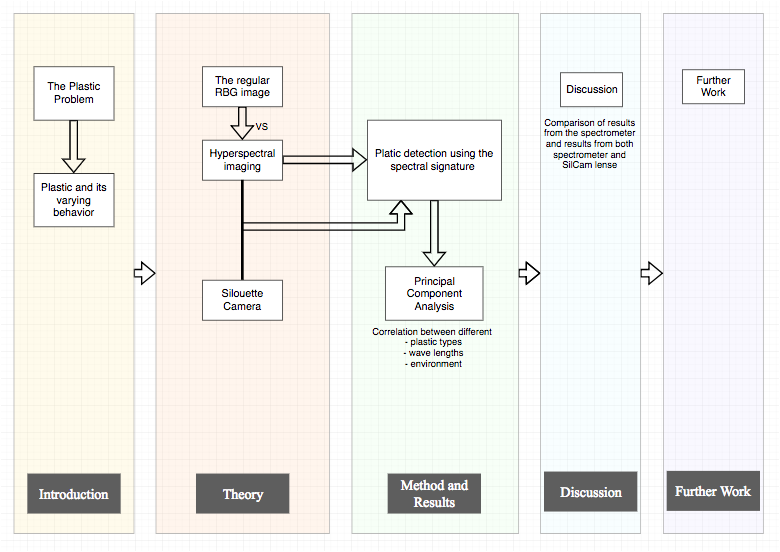
\includegraphics[width=\linewidth]{Images/outline.png}
  \caption{Thesis Outline, roughly sketched}
  \label{fig:outline}
\end{figure}

